\documentclass[border=6pt]{standalone}
\usepackage{tikz}
\usetikzlibrary{arrows.meta,calc}
\begin{document}
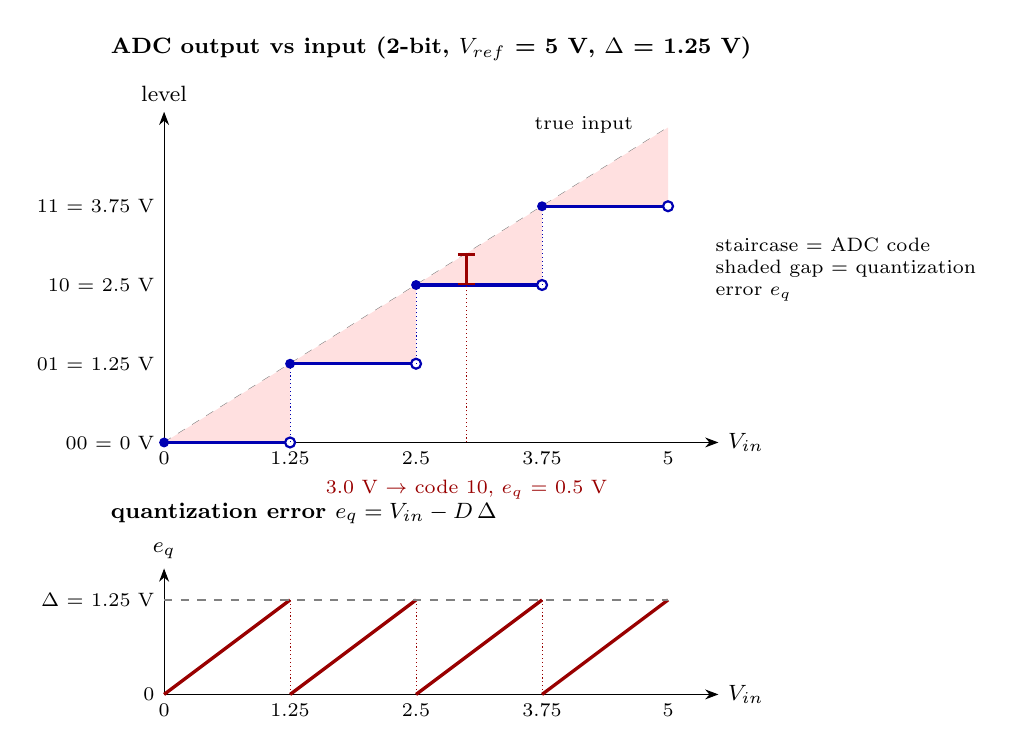
\begin{tikzpicture}[>=Stealth,font=\small,x=1.6cm,y=1cm]
% 2-bit ADC, Vref = 5 V, step 1.25 V, code = floor(Vin/1.25); 1 unit on x = 1.25 V
\node[font=\footnotesize\bfseries,anchor=west] at (-0.5,5.0) {ADC output vs input (2-bit, $V_{ref}$ = 5 V, $\Delta$ = 1.25 V)};
\draw[->] (0,0) -- (4.4,0) node[right,font=\footnotesize]{$V_{in}$};
\draw[->] (0,0) -- (0,4.2) node[above,font=\footnotesize]{level};
\draw[gray,dashed] (0,0) -- (4,4) node[pos=0.95,above left,font=\scriptsize,black]{true input};
\foreach \c/\b in {0/00,1/01,2/10,3/11} {
  \fill[red!12] (\c,\c) -- (\c+1,\c+1) -- (\c+1,\c) -- cycle;
  \draw[very thick,blue!70!black] (\c,\c) -- (\c+1,\c);
  \fill[blue!70!black] (\c,\c) circle (1.8pt);
  \draw[blue!70!black,thick,fill=white] (\c+1,\c) circle (1.8pt);
  \node[anchor=east,font=\scriptsize] at (0,\c) {\b\ = \pgfmathparse{1.25*\c}\pgfmathprintnumber[fixed,precision=2]{\pgfmathresult} V};
}
\foreach \c in {1,2,3} \draw[blue!70!black,densely dotted] (\c,\c-1) -- (\c,\c);
\foreach \x/\l in {0/0,1/1.25,2/2.5,3/3.75,4/5} \node[below,font=\scriptsize] at (\x,0) {\l};
\node[font=\scriptsize,anchor=west,align=left] at (4.3,2.2) {staircase = ADC code\\shaded gap = quantization\\error $e_q$};
% example 3.0 V
\draw[red!60!black,thick,|-|] (2.4,2) -- (2.4,2.4);
\node[font=\scriptsize,red!60!black,anchor=north] at (2.4,-0.35) {3.0 V $\to$ code 10, $e_q$ = 0.5 V};
\draw[red!60!black,densely dotted] (2.4,0) -- (2.4,2);
% error plot
\begin{scope}[yshift=-3.2cm]
\node[font=\footnotesize\bfseries,anchor=west] at (-0.5,2.3) {quantization error $e_q = V_{in} - D\,\Delta$};
\draw[->] (0,0) -- (4.4,0) node[right,font=\footnotesize]{$V_{in}$};
\draw[->] (0,0) -- (0,1.6) node[above,font=\footnotesize]{$e_q$};
\draw[very thick,red!60!black] (0,0) -- (1,1.2) (1,0) -- (2,1.2) (2,0) -- (3,1.2) (3,0) -- (4,1.2);
\foreach \c in {1,2,3} \draw[red!60!black,densely dotted] (\c,1.2) -- (\c,0);
\draw[gray,dashed] (0,1.2) -- (4,1.2);
\node[anchor=east,font=\scriptsize] at (0,1.2) {$\Delta$ = 1.25 V};
\node[anchor=east,font=\scriptsize] at (0,0) {0};
\foreach \x/\l in {0/0,1/1.25,2/2.5,3/3.75,4/5} \node[below,font=\scriptsize] at (\x,0) {\l};
\end{scope}
\end{tikzpicture}
\end{document}
